% Presentación final (Entrega 3), OII464. Compilar en esta carpeta con:
%   latexmk -pdf main.tex
% Regenerar figuras: python figuras/generar_figuras.py
% Comprobar cifras, viñetas y tiempos: python -X utf8 verificar.py
\documentclass[aspectratio=169,11pt]{beamer}
\usepackage[T1]{fontenc}
\usepackage{lmodern}
\usepackage[spanish,es-nodecimaldot,es-noshorthands]{babel}
\usepackage{booktabs,array}
\usepackage{tikz}
\usetikzlibrary{arrows.meta,calc,decorations.pathreplacing,patterns,positioning}

\definecolor{azul}{HTML}{1F4E8C}
\definecolor{azulmedio}{HTML}{4472C4}
\definecolor{azulclaro}{HTML}{E4EBF6}
\definecolor{tinta}{HTML}{1F2933}
\definecolor{gris}{HTML}{5B6673}
\definecolor{grisclaro}{HTML}{D9DEE4}
\definecolor{bloqueo}{HTML}{B5473C}

\setbeamertemplate{navigation symbols}{}
\setbeamertemplate{itemize items}[circle]
\setbeamercolor{normal text}{fg=tinta,bg=white}
\setbeamercolor{structure}{fg=azul}
\setbeamercolor{itemize item}{fg=azulmedio}
\setbeamercolor{frametitle}{fg=azul}
\setbeamerfont{frametitle}{size=\large,series=\bfseries}
\setbeamerfont{caption}{size=\scriptsize}
\setlength{\leftmargini}{1.1em}
\setbeamertemplate{headline}{%
  \begin{tikzpicture}[remember picture,overlay]
    \node[anchor=north east,inner sep=0pt]
      at ($(current page.north east)+(-0.3cm,-0.22cm)$)
      {
\includegraphics[width=2.25cm]{figuras/logo_pucv.png}};
  \end{tikzpicture}}
\setbeamertemplate{frametitle}{%
  \vspace*{0.1cm}%
  \begin{minipage}[t][1.12cm][t]{0.75\paperwidth}
    \raggedright\usebeamerfont{frametitle}\usebeamercolor[fg]{frametitle}\insertframetitle
  \end{minipage}\par
  \vspace{-0.08cm}{\color{azulmedio}\rule{\textwidth}{0.6pt}}\par}
\setbeamertemplate{footline}{%
  \leavevmode\hspace{0.45cm}{\color{gris}\tiny OII464 · Tabu Search + D-MAB}%
  \hfill{\color{gris}\tiny\insertframenumber}\hspace{0.45cm}\vspace{0.2cm}}

\newcommand{\cifra}[3]{%
  \begin{minipage}[t]{0.31\textwidth}\centering
    {\scriptsize\color{gris}#1\par}\vspace{0.1cm}
    {\LARGE\bfseries\boldmath\color{azul}#2\par}\vspace{0.1cm}
    {\scriptsize #3\par}
  \end{minipage}}
\newcommand{\recuadro}[2]{%
  \begin{tikzpicture}
    \node[fill=azulclaro,text width=0.96\textwidth,inner sep=7pt,align=left] {%
      {\small\bfseries\color{azul} #1}\\[0.08cm] #2};
  \end{tikzpicture}}

% Beamer no admite macros con parámetros definidas dentro de un frame.
\newcommand{\fila}[2]{\node[anchor=east,text=gris] at (-0.1,#1+0.4) {#2};}
\newcommand{\tramo}[4]{\fill[#4] (#1,0) rectangle (#2,1);
  \node[align=center] at ({(#1+#2)/2},0.5) {#3};}
\newcommand{\detalle}[5]{\fill[#4] (#1,0) rectangle (#2,1);
  \node[align=center,text=#5] at ({(#1+#2)/2},0.5) {#3};}

\title{Programación de cirugías electivas mediante búsqueda tabú y selección adaptativa de movimientos}
\author{José Basualto, Cristopher Dauros y Carlos Ruz}
\date{Noviembre de 2026}

\begin{document}

\begin{frame}[plain]
  \begin{tikzpicture}[remember picture,overlay]
    \node[anchor=north,inner sep=0pt] at (current page.north)
      {
\includegraphics[width=\paperwidth]{figuras/encabezado.png}};
  \end{tikzpicture}
  \vspace*{3.75cm}
  \begin{center}
    {\Large\bfseries\color{azul} Programación de cirugías electivas mediante búsqueda tabú y selección adaptativa de movimientos\par}
    \vspace{0.18cm}
    {\normalsize Informe final: resultados y conclusiones\par}
    \vspace{0.18cm}
    {\small José Basualto · Cristopher Dauros · Carlos Ruz\par}
    \vspace{0.05cm}
    {\scriptsize\color{gris} OII464: Desarrollo de Diseños Híbridos para Optimización · Prof. Emanuel Vega · Noviembre de 2026\par}
  \end{center}
\end{frame}

% ---------- Introducción: problema, vacío y pregunta ----------

\begin{frame}{Mientras un paciente espera, su sala y su anestesista quedan bloqueados}
  \centering
  \begin{tikzpicture}[x=1cm,y=0.55cm,font=\scriptsize]
    \fila{3}{Sala de anestesia}
    \fila{2}{Anestesista}
    \fila{1}{Sala de cirugía}
    \fila{0}{Cirujano}
    \foreach \y in {3,2}{
      \fill[azulmedio] (0,\y) rectangle (3.4,\y+0.8);
      \node[text=white] at (1.7,\y+0.4) {Anestesia};
    }
    \foreach \y/\etiqueta in {3/Bloqueada,2/Reservado}{
      \fill[bloqueo!12] (3.4,\y) rectangle (5.6,\y+0.8);
      \fill[pattern=north east lines,pattern color=bloqueo] (3.4,\y) rectangle (5.6,\y+0.8);
      \node[fill=white,inner sep=1pt,text=bloqueo] at (4.5,\y+0.4) {\etiqueta};
    }
    \foreach \y in {1,0}{
      \fill[grisclaro] (0,\y) rectangle (5.6,\y+0.8);
      \node[text=gris] at (1.7,\y+0.4) {Paciente anterior};
      \fill[azulmedio] (5.6,\y) rectangle (10.2,\y+0.8);
      \node[text=white] at (7.9,\y+0.4) {Cirugía};
    }
    \draw[gris,dashed] (3.4,-0.15) -- (3.4,4.05);
    \draw[gris,dashed] (5.6,-0.15) -- (5.6,4.05);
    \draw[decorate,decoration={brace,amplitude=4pt},thick,bloqueo]
      (3.4,4.1) -- (5.6,4.1) node[midway,above=3pt] {Espera $W_j$};
    \draw[-{Latex},gris] (0,-0.35) -- (10.5,-0.35) node[midway,below] {Tiempo (esquema conceptual)};
  \end{tikzpicture}

  \vspace{0.08cm}
  \begin{itemize}
    \item La anestesia termina, pero la sala de cirugía sigue ocupada.
    \item La primera sala y el anestesista quedan retenidos hasta el traslado.
    \item Ese bloqueo retrasa a los pacientes siguientes y alarga la jornada.
  \end{itemize}
\end{frame}

\begin{frame}{El calendario debe terminar antes sin exceder la espera máxima}
  \begin{itemize}
    \item Cada paciente pasa por anestesia y luego por cirugía.
    \item El planificador asigna personal e inicia cada etapa lo antes posible.
    \item Restricción estricta: la espera nunca supera \texttt{max\_wait}.
    \item Minimizamos un objetivo combinado, sin penalizar desequilibrio de salas.
  \end{itemize}
  \vspace{0.25cm}
  \[
    f(S)=
    \underbrace{C_{\max}}_{\text{fin de la jornada}}
    +\underbrace{10^{-6}\sum_{o} t_o^{\mathrm{ini}}}_{\text{desempate}}
    +\underbrace{0{,}5\sum_{j} W_j}_{\text{espera total}}
    +\underbrace{1{,}4\max_{j} W_j}_{\text{peor espera}}
  \]
\end{frame}

\begin{frame}{Faltaba separar el aporte de D-MAB en Tabu con espera estricta}
  \begin{itemize}
    \item Yu et al. (2024): Q-learning en programación quirúrgica.
    \item Dolatkhah et al. (2026, preprint): D-MAB dentro de un genético.
    \item Yin et al. (2026): Tabu multioperador entre hospitales.
    \item Vacío en lo revisado: separar selección, cómputo y repetición.
  \end{itemize}
  \vspace{0.25cm}
  \recuadro{Pregunta de investigación}{%
    ¿En qué condiciones D-MAB mejora Tabu Search frente a la selección uniforme
    de los mismos movimientos?}
\end{frame}

% ---------- Propuesta ----------

\begin{frame}{Una cartera fija corre dos caminos y conserva el mejor calendario}
  \centering
  \begin{tikzpicture}[font=\scriptsize,
      caja/.style={draw=azulmedio,fill=azulclaro,rounded corners=2pt,align=center,
                   minimum height=0.95cm,inner sep=4pt},
      aprende/.style={caja,fill=azulmedio,text=white,draw=azul},
      flecha/.style={-{Latex},gris,thick}]
    \node[caja,text width=1.55cm] (datos) {Instancia validada};
    \node[caja,text width=2.15cm,right=0.5cm of datos] (ini) {30 soluciones iniciales\\FIFO, SPT, LPT\\y 27 aleatorias};
    \node[caja,text width=2.9cm,above right=0.05cm and 0.75cm of ini.east,anchor=south west] (uni) {Tabu uniforme\\3.030 evaluaciones};
    \node[aprende,text width=2.9cm,below right=0.05cm and 0.75cm of ini.east,anchor=north west] (dmab) {Tabu + D-MAB\\3.030 evaluaciones};
    \node[caja,text width=2.05cm,right=4.75cm of ini] (min) {Menor $f$ factible\\(desempata por $C_{\max}$)};
    \draw[flecha] (datos) -- (ini);
    \draw[flecha] (ini.east) -- (uni.west);
    \draw[flecha] (ini.east) -- (dmab.west);
    \draw[flecha] (uni.east) -- (min.west);
    \draw[flecha] (dmab.east) -- (min.west);
    \node[below=0.06cm of dmab,text=azul] {ML: fase de evolución};
  \end{tikzpicture}

  \vspace{0.32cm}
  \begin{itemize}
    \item ML actúa en la fase de evolución: elige cada movimiento.
    \item Reparto 50/50 y selección final son deterministas.
    \item No empeora el Tabu de 3.030 de su semilla; gasta el doble.
  \end{itemize}
\end{frame}

\begin{frame}{D-MAB aprende en línea qué movimiento proponer a Tabu}
  \[
    a_t=\arg\max_{a}\left[\bar r_a+c\sqrt{\frac{2\ln n}{n_a}}\right],
    \qquad c=0{,}1
  \]
  \begin{itemize}
    \item Cinco brazos: \texttt{swap}, \texttt{insert}, \texttt{room\_1}, \texttt{room\_2}, \texttt{room\_pair}.
    \item Recompensa: mejora del candidato frente al estado local previo.
    \item UCB1 equilibra la recompensa media y la exploración.
    \item Page--Hinkley detecta caídas y reinicia las estadísticas del bandido.
    \item D-MAB es UCB1 más ese reinicio; sin él queda UCB1.
  \end{itemize}
\end{frame}

% ---------- Configuración experimental ----------

\begin{frame}{Cuatro comparaciones separan selección, cómputo y repetición de la búsqueda}
  \centering\footnotesize
  \begin{tabular}{@{}lll@{}}
    \toprule
    Id & Comparación (evaluaciones) & Explicación alternativa que descarta\\
    \midrule
    C1 & D-MAB $-$ Tabu uniforme (3.030) & La mejora viene de Tabu, no de la selección\\
    C2 & Cartera $-$ Tabu prolongado (6.060) & La cartera mejora solo por más evaluaciones\\
    C3 & Cartera $-$ dos Tabu (6.060) & La cartera mejora por repetir la búsqueda\\
    C4 & D-MAB $-$ UCB1 sin reinicio (3.030) & El efecto viene de UCB1, no del reinicio\\
    \bottomrule
  \end{tabular}

  \vspace{0.3cm}
  \raggedright\normalsize
  \begin{itemize}
    \item Wilcoxon sobre medias por instancia, Holm sobre C1--C4, bootstrap jerárquico.
    \item Signo: alternativa $-$ referencia; negativo favorece a la alternativa.
    \item Umbral mínimo: 0,25 de $f$, sin significado clínico.
    \item Regla para C1: $p$ Holm $<0{,}05$, IC bajo cero y media $\le -0{,}25$.
  \end{itemize}
\end{frame}

\begin{frame}{El catálogo de congestión tensiona la espera que el original no tensionaba}
  \begin{columns}[c,onlytextwidth]
    \begin{column}{0.53\textwidth}
      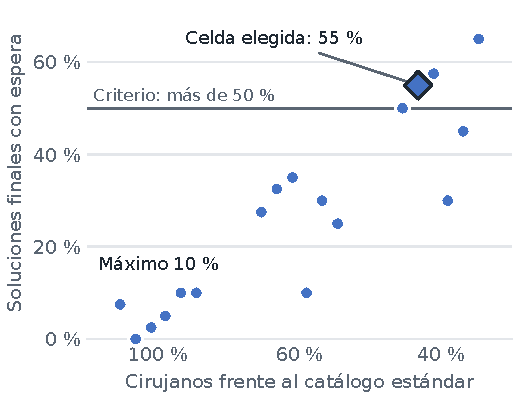
\includegraphics[width=\linewidth]{figuras/calibracion_espera.pdf}
    \end{column}
    \begin{column}{0.44\textwidth}
      \small
      \begin{itemize}
        \item Catálogo estándar: solo 16 de 240 soluciones con espera.
        \item Reducir salas o \texttt{max\_wait} dejó 10 \% o menos.
        \item Reducir cirujanos al 40 \% alcanzó 55 \% en desarrollo.
        \item Catálogo final: 48 instancias nuevas, sintéticas.
        \item En ellas, 51,8 \% de las soluciones terminó con espera.
      \end{itemize}
    \end{column}
  \end{columns}
\end{frame}

\begin{frame}{Dos protocolos fijaron semillas, tamaño y regla antes de ejecutar}
  \centering
  \begin{tikzpicture}[x=0.098cm,y=0.85cm,font=\fontsize{7.2}{8.4}\selectfont]
    \tramo{0}{80}{Estudios previos\\semillas 0--79}{azulclaro}
    \fill[azulmedio] (80.4,0) rectangle (120,1);
    \node[text=white,align=center] at (100.2,0.5) {Entrega 2\\80--119};
    \fill[azul] (120.4,0) rectangle (140,1);
    \node[text=white,align=center] at (130.2,0.5) {Confirmación\\120--139};
    \draw[gris] (80.4,0) -- (0,-0.45);
    \draw[gris] (120,0) -- (140,-0.45);
    \begin{scope}[x=0.343cm,shift={(0,-1.45)}]
      \detalle{0}{4.9}{Tiempos\\80--84}{azulclaro}{tinta}
      \detalle{5.1}{9.9}{Calibración\\85--89}{azulclaro}{tinta}
      \detalle{10.1}{29.9}{Estudio de congestión C1--C4\\90--109}{azulmedio}{white}
      \detalle{30.1}{34.9}{Piloto\\110--114}{azulclaro}{tinta}
      \detalle{35.1}{40}{Diagnóstico\\115--119}{azulclaro}{tinta}
    \end{scope}
  \end{tikzpicture}

  \vspace{0.2cm}
  \raggedright
  \begin{itemize}
    \item Hipótesis, pruebas y regla quedaron en commits previos a cada estudio.
    \item Tamaño fijado: 48 instancias por 20 semillas, 960 pares.
    \item Potencia simulada para detectar 0,65: 0,87.
    \item Con la variabilidad observada, esa potencia aproximada baja a 0,32.
  \end{itemize}
\end{frame}

% ---------- Resultados ----------

\begin{frame}{La hipótesis primaria no queda respaldada: el intervalo de C1 incluye el cero}
  \centering
  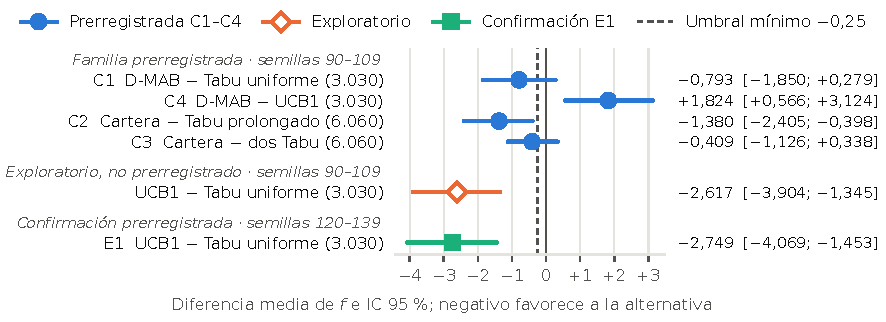
\includegraphics[width=\textwidth]{figuras/forest_comparaciones.pdf}

  \vspace{0.05cm}
  \raggedright\small
  \begin{itemize}
    \item Validez: 960 pares sin fallos y 5.760 calendarios auditados.
    \item C1 cumple dos de tres condiciones, también por base: no concluyente.
  \end{itemize}
\end{frame}

\begin{frame}{La ganancia de la cartera es compatible con repetir la búsqueda}
  \centering
  \cifra{C2: cartera $-$ Tabu prolongado}{$-1{,}380$}{IC [$-2{,}405$; $-0{,}398$]\\$p$ Holm 0,008}\hfill
  \cifra{C3: cartera $-$ dos Tabu}{$-0{,}409$}{IC [$-1{,}126$; $+0{,}338$]\\$p$ Holm 0,057}\hfill
  \cifra{Tabu prolongado sin mejoras tras 3.030}{56,9 \%}{546 de 960 corridas\\(descriptivo)}

  \vspace{0.4cm}
  \raggedright
  \begin{itemize}
    \item Superó al prolongado, pero por base pierde significación.
    \item La ventaja solo aparece con 25 y 30 cirugías.
    \item No distinguimos la cartera de dos Tabu uniformes.
    \item Por tanto, no atribuimos esa ganancia al aprendizaje.
    \item Cautela: el error tipo I simulado de C2 fue 0,082.
  \end{itemize}
\end{frame}

\begin{frame}{El reinicio Page--Hinkley no ayudó bajo congestión}
  \centering
  \cifra{C4: D-MAB $-$ UCB1 sin reinicio}{$+1{,}824$}{IC [$+0{,}566$; $+3{,}124$]\\$p$ Holm 0,005}\hfill
  \cifra{Reinicios por corrida (mediana)}{24}{uno cada 126 evaluaciones\\(descriptivo)}\hfill
  \cifra{Reinicios aunque nada cambie}{25}{simulación, brazos idénticos\\(diagnóstico exploratorio)}

  \vspace{0.4cm}
  \raggedright
  \begin{itemize}
    \item D-MAB perdió ante UCB1; por base, no es significativo.
    \item Con 15 cirugías, en cambio, D-MAB fue mejor en media.
    \item El 59,3 \% de los reinicios ocurre con recompensa ya estable.
    \item Con $\lambda=1$, el ruido basta para disparar el detector.
    \item El brazo líder causó 96,8 \% de los reinicios.
  \end{itemize}
\end{frame}

\begin{frame}{Una confirmación prerregistrada respaldó a UCB1 frente a Tabu uniforme}
  \centering
  \cifra{E1: UCB1 sin reinicio $-$ Tabu uniforme}{$-2{,}749$}{IC [$-4{,}069$; $-1{,}453$]\\$p<0{,}001$}\hfill
  \cifra{Semillas nuevas 120--139}{960 pares}{48 instancias de congestión,\\sin fallos}\hfill
  \cifra{Auditoría}{1.920}{calendarios finales\\recalculados}

  \vspace{0.4cm}
  \raggedright
  \begin{itemize}
    \item El contraste exploratorio previo, $-2{,}617$, era solo una hipótesis.
    \item Registramos protocolo, regla y tamaño antes de ejecutar.
    \item E1 cumple la regla, también al analizar por base.
    \item Con 15 cirugías no hay ventaja: $+0{,}12$.
    \item No evalúa una cartera con UCB1 ni otros hospitales.
  \end{itemize}
\end{frame}

% ---------- Discusión y conclusión ----------

\begin{frame}{Ayuda UCB1 bajo congestión, con costo y sin probar aprendizaje}
  \begin{columns}[t,onlytextwidth]
    \begin{column}{0.48\textwidth}
      {\bfseries\color{azul} Qué explica el resultado}
      \begin{itemize}
        \item DaCosta et al.: sin reinicio ganó con recompensas binarias.
        \item Reparación: afecta a todos; en D-MAB, 44,0 \%.
        \item UCB1 pudo solo sesgar movimientos: falta mezcla fija.
      \end{itemize}
    \end{column}
    \begin{column}{0.48\textwidth}
      {\bfseries\color{azul} Qué limita la conclusión}
      \begin{itemize}
        \item UCB1 tardó 10,2 \% más y varió más.
        \item Vale con inicios lo antes posible; en el estándar cambian los signos.
      \end{itemize}
    \end{column}
  \end{columns}
\end{frame}

\begin{frame}{D-MAB completo no mejora de forma concluyente; aporta UCB1 sin reinicio}
  \recuadro{Respuesta a la pregunta}{%
    No identificamos una condición en que D-MAB completo mejore de forma concluyente
    a Tabu uniforme. Bajo congestión y con inicios lo antes posible, sí aporta UCB1 sin reinicio.}

  \vspace{0.2cm}
  \begin{itemize}
    \item Solo E1 resiste el reanálisis exploratorio por instancia base.
    \item Aporte: controles a igual presupuesto y dos protocolos prerregistrados.
    \item Futuro: mezcla fija, recompensa global y $\lambda$ recalibrado.
    \item Futuro: cartera con UCB1 frente a dos Tabu independientes.
    \item Futuro: instancias reservadas, mayor tamaño y comparación a igual tiempo.
  \end{itemize}
\end{frame}

\appendix

\begin{frame}{Apéndice: la configuración quedó congelada antes de ejecutar}
  \centering\footnotesize
  \begin{tabular}{@{}p{0.17\textwidth}p{0.78\textwidth}@{}}
    \toprule
    Componente & Configuración\\
    \midrule
    Tabu & 30 soluciones iniciales (FIFO, SPT, LPT y 27 aleatorias); lotes de 15 candidatos; memoria de 7 firmas de solución; aspiración por mejora global.\\
    D-MAB & Cinco brazos; $c=0{,}1$; $\delta=0{,}01$; $\lambda=1$.\\
    Cartera & Dos caminos de 3.030 evaluaciones; reparto 50/50 fijo; conserva el menor $f$.\\
    Parada & Agotar el presupuesto de evaluaciones del camino.\\
    Conteo & Cuentan las 30 iniciales y cada candidato distinto del lote, aun infactible. No cuentan duplicados, reparación ni revalidación final.\\
    Entorno & AMD Ryzen 7 8845HS, 8 núcleos, 13,8 GiB; Python 3.13.2, NumPy 2.2.3, SciPy 1.15.2.\\
    \bottomrule
  \end{tabular}
\end{frame}

\begin{frame}{Apéndice: la regla de C1 y la potencia del estudio}
  \begin{itemize}
    \item Regla: $p$ Holm $<0{,}05$, IC completo bajo cero y media $\le -0{,}25$.
    \item C1: media $-0{,}793$, IC [$-1{,}850$; $+0{,}279$], $p$ Holm 0,041.
    \item Planificación: DE supuesta 7,03 y potencia simulada 0,87.
    \item Realidad: DE observada 13,21 y potencia aproximada 0,32.
    \item Detectar 0,65 con esa DE pediría 3.246 pares.
  \end{itemize}
\end{frame}

\begin{frame}{Apéndice: por instancia base, solo E1 cumple la regla}
  \centering\footnotesize
  Semillas 90--109\par\smallskip
  \begin{tabular}{@{}lcrl@{}}
    \toprule
    Comparación & IC 95 \% & $p$ Holm & Regla\\
    \midrule
    C1: D-MAB $-$ uniforme & [$-1{,}786$; $+0{,}176$] & 0,010 & No cumple\\
    C2: cartera $-$ prolongado & [$-2{,}844$; $+0{,}123$] & 0,192 & No cumple\\
    C3: cartera $-$ dos Tabu & [$-1{,}124$; $+0{,}288$] & 0,204 & No cumple\\
    C4: D-MAB $-$ UCB1 & [$+0{,}085$; $+3{,}566$] & 0,192 & No cumple\\
    \bottomrule
  \end{tabular}

  \bigskip
  Semillas 120--139\par\smallskip
  \begin{tabular}{@{}lcrl@{}}
    \toprule
    Comparación & IC 95 \% & $p$ & Regla\\
    \midrule
    E1: UCB1 $-$ uniforme & [$-4{,}335$; $-1{,}191$] & 0,005 & Cumple\\
    \bottomrule
  \end{tabular}

  \bigskip
  {\scriptsize Exploratorio, decidido tras ver los resultados: 12 bases como unidad.
  No cambia las decisiones registradas.}
\end{frame}

\begin{frame}{Apéndice: el protocolo de la confirmación E1 se registró antes de correr}
  \centering\footnotesize
  \begin{tabular}{@{}p{0.2\textwidth}p{0.75\textwidth}@{}}
    \toprule
    Elemento & Definición registrada\\
    \midrule
    Comparación & Una sola: UCB1 sin reinicio $-$ Tabu uniforme, 3.030 evaluaciones.\\
    Datos y semillas & Las 48 instancias de congestión; semillas nuevas 120--139.\\
    Prueba & Wilcoxon sobre medias por instancia; sin corrección múltiple.\\
    Incertidumbre & Bootstrap jerárquico de instancias y semillas, 5.000 réplicas.\\
    Regla & La misma de C1: $p<0{,}05$, IC bajo cero y media $\le -0{,}25$.\\
    Tamaño & 960 pares fijados de antemano; sin parada opcional.\\
    Registro & Protocolo en el commit \texttt{05ca74a}, anterior a la ejecución.\\
    \bottomrule
  \end{tabular}
\end{frame}

\begin{frame}{Apéndice: calidad absoluta, dispersión y tiempo en congestión}
  \centering\footnotesize
  \begin{tabular}{@{}lrrrrrr@{}}
    \toprule
    Método (evaluaciones) & Mejor & Media & Peor & DE & RPD (\%) & $t$ (s)\\
    \midrule
    Uniforme (3.030) & 280,31 & 297,20 & 312,80 & 8,72 & 9,75 & 6,17\\
    D-MAB (3.030) & 279,32 & 296,40 & 312,88 & 8,85 & 9,46 & 6,51\\
    UCB1 (3.030) & 277,21 & 294,58 & 311,79 & 9,36 & 8,79 & 6,77\\
    Prolongado (6.060) & 277,81 & 293,23 & 307,97 & 7,95 & 8,25 & 12,43\\
    Dos Tabu (6.060) & 277,87 & 292,26 & 305,89 & 7,29 & 7,89 & 12,59\\
    Cartera (6.060) & 277,15 & 291,85 & 304,91 & 7,29 & 7,76 & 12,87\\
    \bottomrule
  \end{tabular}

  \vspace{0.15cm}
  {\scriptsize Semillas 90--109. RPD: respecto del mejor valor conocido, no del óptimo.}
\end{frame}

\begin{frame}{Apéndice: en el catálogo estándar los signos no son consistentes}
  \centering\footnotesize
  Semillas 20--39, configuración anterior\par\smallskip
  \begin{tabular}{@{}ccc@{}}
    \toprule
    UCB1 $-$ uniforme & D-MAB $-$ uniforme & D-MAB $-$ UCB1\\
    \midrule
    $-0{,}455$ & $-0{,}513$ & $-0{,}058$\\
    \bottomrule
  \end{tabular}

  \bigskip
  Semillas 40--59, configuración vigente\par\smallskip
  \begin{tabular}{@{}ccc@{}}
    \toprule
    UCB1 $-$ uniforme & D-MAB $-$ uniforme & D-MAB $-$ UCB1\\
    \midrule
    $+1{,}182$ & $+0{,}577$ & $-0{,}605$\\
    \bottomrule
  \end{tabular}

  \bigskip
  {\scriptsize Descriptivo, 12 instancias. Son estudios distintos y no se combinan.}
\end{frame}

\begin{frame}{Apéndice: en las oficiales la cartera supera a las reglas}
  \centering\footnotesize
  Frente a la mejor de FIFO, SPT y LPT; semillas 60--79, 6.060 evaluaciones\par\smallskip
  \begin{tabular}{@{}lcc@{}}
    \toprule
    Medida & Cartera & Dos Tabu\\
    \midrule
    Instancias ganadas en $f$ & 12 de 12 & 12 de 12\\
    Reducción media de $f$ & 5,89 \% & 5,90 \%\\
    Ganadas en \emph{makespan} & 10 de 12 & 10 de 12\\
    Ganadas con penalización por desequilibrio & 10 de 12 & 10 de 12\\
    \bottomrule
  \end{tabular}

  \bigskip
  {\scriptsize Exploratorio. Dos Tabu logran lo mismo: no lo atribuimos al aprendizaje.}
\end{frame}

\begin{frame}{Apéndice: al retrasar la anestesia desaparece la espera}
  \begin{itemize}
    \item El planificador, como el simulador docente, inicia lo antes posible.
    \item Retrasar solo la anestesia deja la espera en cero.
    \item Entonces la mejor regla gana en las 48 instancias.
    \item La ventaja de UCB1 baja a 1,656 (E1) y 0,093 (90--109).
    \item Exploratorio: no repetimos la búsqueda con esa regla.
  \end{itemize}
\end{frame}

\end{document}
